\documentclass[12pt,a4paper]{beamer}
\usepackage[utf8]{inputenc}
\usepackage{amsmath}
\usepackage{amsfonts}
\usepackage{amssymb, multicol}
\usepackage{framed}

\usepackage{graphicx}
\usepackage{caption}
\usepackage{subcaption}

\begin{document}
\begin{frame}{Linear regression}
	Linear regression assumes that the relationship between two variables, $x$ and $y$, can be modelled by a straight line:
	\begin{eqnarray*}
	y = \beta_0 + \beta_1x
	\end{eqnarray*}
	where $\beta_0$ is the intercept and $\beta_1$ the slope.
	\vspace{0.1cm}
	
	\begin{itemize}
		\item $x$ is called the \textbf{explanatory} or the \textbf{predictor} variable,
		\item $y$ is called the \textbf{response} variable.
	\end{itemize}
	
	
\end{frame}
\begin{frame}{Linear regression}
	\textbf{Theory}
	\begin{figure}
	   \centering
	   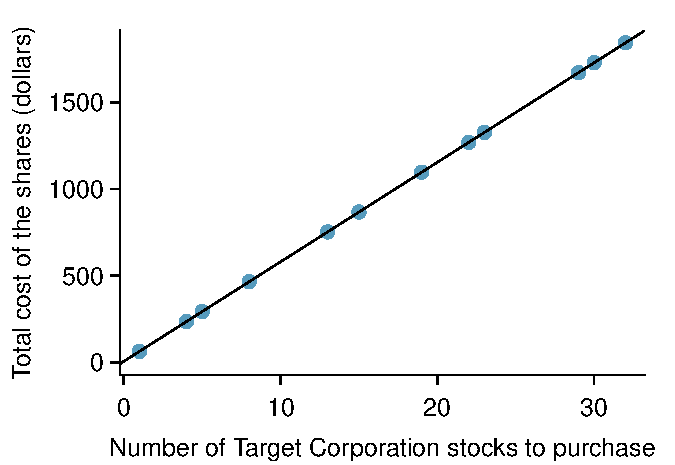
\includegraphics[width=0.4\textwidth]{figures/perfLinearModel/perfLinearModel}
	\end{figure}
	\textbf{Reality}
	\begin{figure}
	   \centering
	   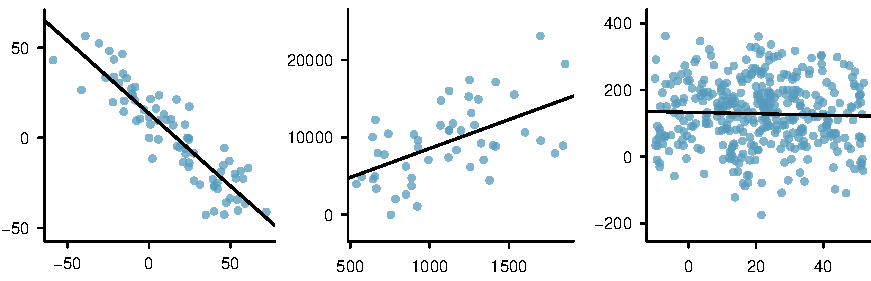
\includegraphics[width=0.8\textwidth]{figures/imperfLinearModel/imperfLinearModel}
	   \label{imperfLinearModel}
	\end{figure}
\end{frame}
	\begin{frame}{Look for linear trend}
		Examine the \textbf{scatter plot}
		\begin{figure}
		   \centering
		   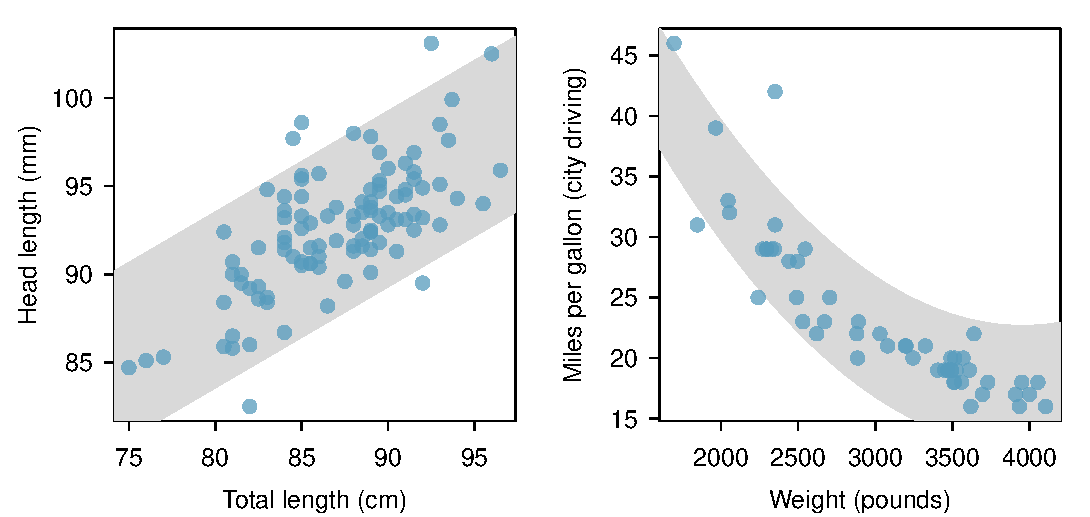
\includegraphics[width=\textwidth]{figures/scattHeadLTotalLTube/scattHeadLTotalLTube}
		\end{figure}
	\end{frame}
	\begin{frame}{Fitting a line}
		\begin{figure}
		   \centering
		   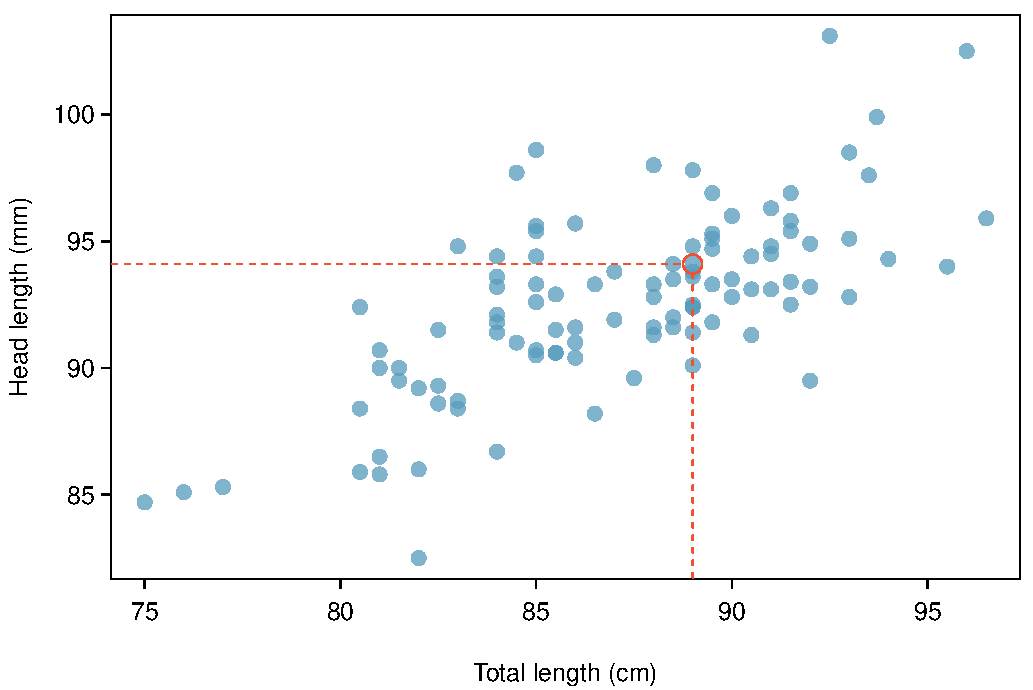
\includegraphics[width=0.7\textwidth]{figures/scattHeadLTotalL/scattHeadLTotalL}
		   \caption{\small A scatterplot showing head length against total length for 104 brushtail possums. A point representing a possum with head length 94.1mm and total length 89cm is highlighted.}
		   \label{scattHeadLTotalL}
		\end{figure}
	\end{frame}
	\begin{frame}{Fitting a line}
		\textbf{Probabilistic interepretation}\\
		\[y=\beta_0+\beta_1x+\epsilon,\]
		where $\epsilon$ is a random variable with mean 0.
	
	The fitted line
	\[\hat{y}=b_0+b_1x,\]
	 is the expected value of y  for fixed x.
	 \end{frame}
	\begin{frame}{Residuals}
		\textbf{Residuals} are the leftover variation in the data after accounting for the model fit:
		\begin{align*}
		\text{Data} = \text{Fit} + \text{Residual}
		\end{align*}
		\begin{framed}
			The residual of the $i^{th}$ observation $(x_i, y_i)$ is the difference of the observed response ($y_i$) and the response we would predict based on the model fit ($\hat{y}_i$):
			\begin{eqnarray*}
			e_i = y_i - \hat{y}_i
			\end{eqnarray*}
			We typically identify $\hat{y}_i$ by plugging $x_i$ into the model.
		\end{framed}
	\end{frame}
	\begin{frame}{Residuals}
		\begin{figure}
		   	\centering
			\begin{minipage}{.5\textwidth}
			  \centering
		   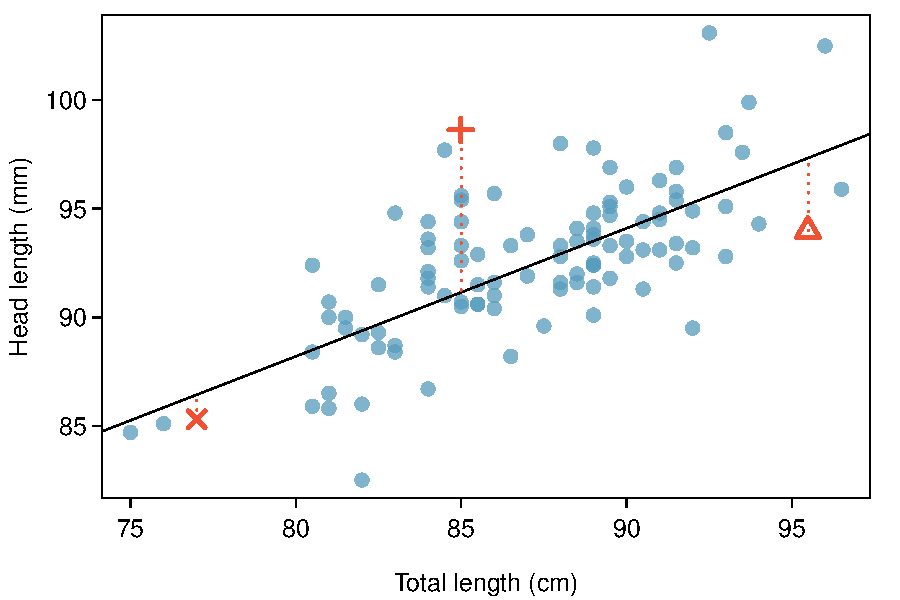
\includegraphics[width=\textwidth]{figures/scattHeadLTotalLLine/scattHeadLTotalLLine}
		   
	\end{minipage}%
	\begin{minipage}{0.4\textwidth}
	\small	Fitted line:
		\[\hat{y}=41+0.59x\]
		Observations:
\small
		\begin{itemize}
			\item $\times$ is $(77.0, 85.3)$ $\Rightarrow$ $e_{\times}=y_{\times}-(41+0.59x_{\times})=-1.1$
			\item $+$ is 	$(85.0, 98.6)$ $\Rightarrow$ $e_{+}=y_{+}-\hat{y}_{+}=7.45$
			\item $\triangle$ is  $(95.5, 94.0)$ $\Rightarrow$ $e_{\triangle}=y_{\triangle}-\hat{y}_{\triangle}=-3.3$
		\end{itemize}
	\end{minipage}
				\end{figure}
		\end{frame}
\begin{frame}{Residual plot}
	
	\begin{figure}
	   \centering
	   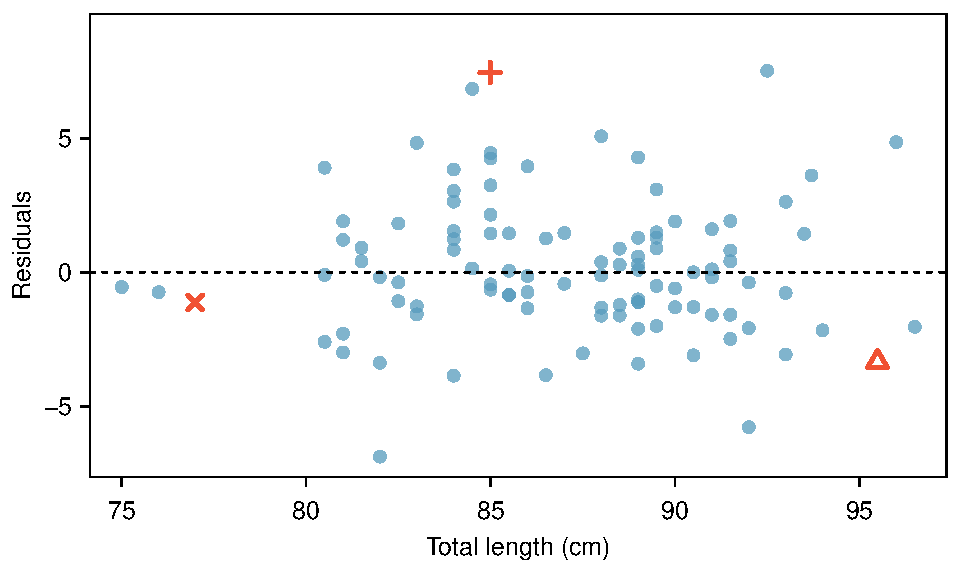
\includegraphics[width=0.73\textwidth]{figures/scattHeadLTotalLResidualPlot/scattHeadLTotalLResidualPlot}
	   
	\end{figure}
\end{frame}
\begin{frame}{Residual plots-Linear models}
	\textbf{Q:} How well does a linear model fit the data?
	\begin{figure}
	   \centering
	   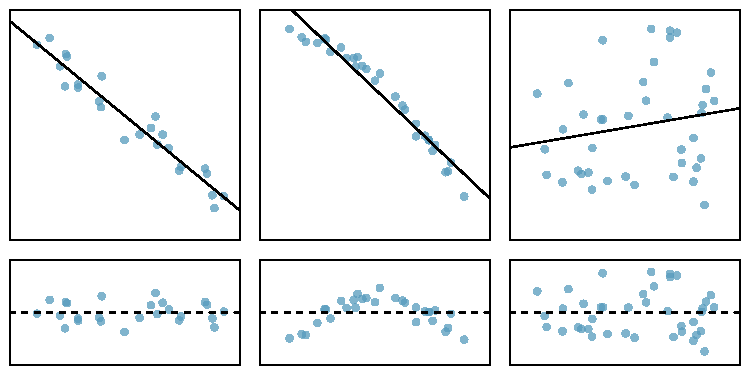
\includegraphics[width=\textwidth]{figures/sampleLinesAndResPlots/sampleLinesAndResPlots}
	   \caption{Sample data with their best fitting lines (top row) and their corresponding residual plots (bottom row).}
	\end{figure}
\end{frame}
\begin{frame}{Correlation $R$}
	\begin{framed}
\textbf{Correlation}, which always takes values between -1 and 1, describes the \textit{strength of the linear relationship} between two variables. We denote the correlation by $R$.
	\end{framed}
	\begin{framed}
		\textbf{Formally:}\\
		The \textbf{correlation}, $R$, for observations $(x_1, y_1)$, $(x_2, y_2)$, ..., $(x_n, y_n)$ is:
		\begin{eqnarray*}
		R = \frac{1}{n-1}\sum_{i=1}^{n} \frac{x_i-\bar{x}}{s_x}\frac{y_i-\bar{y}}{s_y}
		\end{eqnarray*}
		where $\bar{x}$, $\bar{y}$, $s_x$, and $s_y$ are the sample means and standard deviations for each variable.
	\end{framed}
\end{frame}
\begin{frame}{Correlation}
	\begin{figure}
	   \centering
	   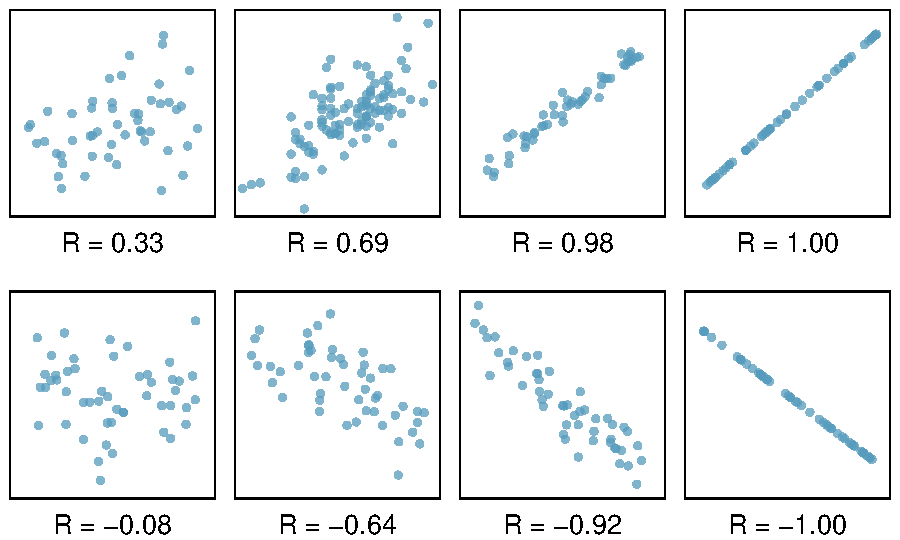
\includegraphics[width=0.85\textwidth]{figures/posNegCorPlots/posNegCorPlots}
	  \small \caption{Sample scatterplots and their correlations. The first row shows variables with a positive relationship, represented by the trend up and to the right. The second row shows variables with a negative trend, where a large value in one variable is associated with a low value in the other.}
	\end{figure}
\end{frame}
\begin{frame}{Correlation}
	The correlation quantifies the strength of a \textbf{linear} trend!!!! 
	\begin{figure}
	   \centering
	   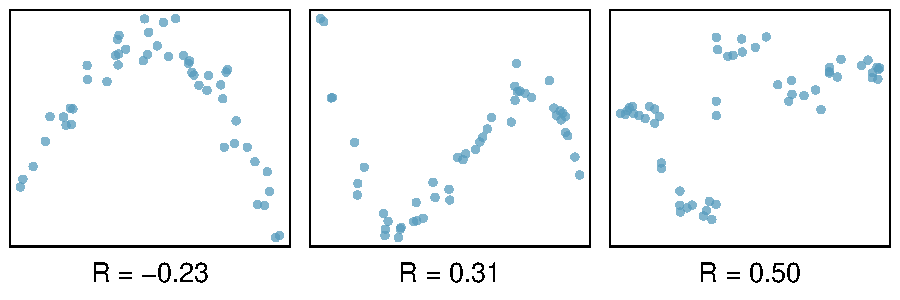
\includegraphics[width=0.86\textwidth]{figures/posNegCorPlots/corForNonLinearPlots}
	   \small\caption{Sample scatterplots and their correlations. In each case, there is a strong relationship between the variables. However, the correlation is not very strong, and the relationship is not linear.}
	\end{figure}
\end{frame}
\begin{frame}{Correlation}
\begin{figure}
	\centering
	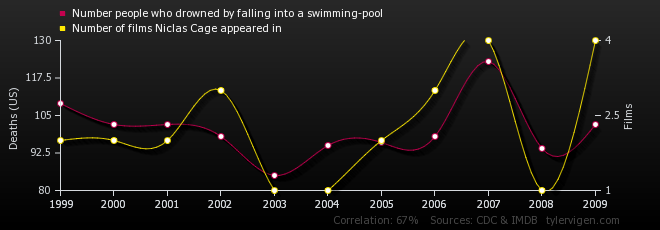
\includegraphics[width=\textwidth]{figures/Correlation}
	\end{figure}
	$R=0.66$\footnote{http://tylervigen.com/}
\end{frame}
\begin{frame}{Fitting a line}
	Which line is optimal?
	\begin{figure}
	\centering
	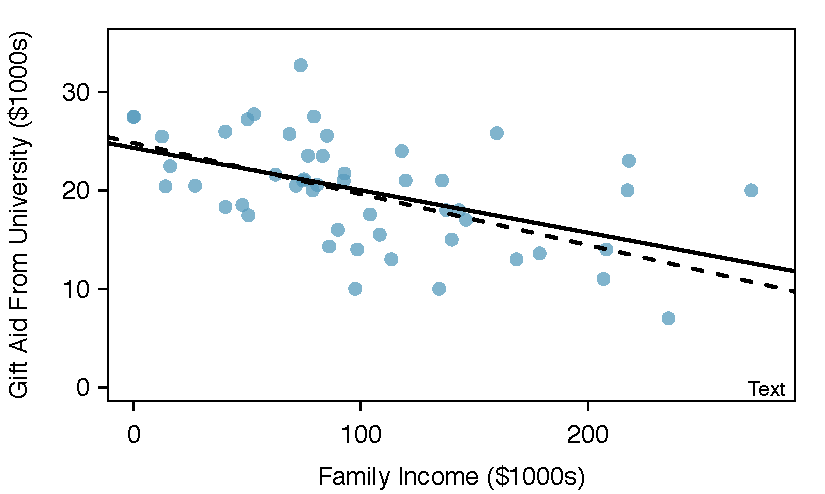
\includegraphics[width=0.75\textwidth]{figures/elmhurstPlots/elmhurstScatterW2Lines}
	\caption{\small Gift aid and family income for a random sample of 50 freshman students from Elmhurst College. Two lines are fit to the data, the solid line being the \emph{least squares line}.}
	\label{elmhurstScatterW2Lines}
	\end{figure}
\end{frame}
\begin{frame}{Conditions }
	\begin{itemize}
		\item \textbf{Linearity} The data should show a linear trend. 
		\item \textbf{Nearly normal residuals} The residuals must be nearly normal.
		When this condition is found to be unreasonable, it is usually because of outliers or concerns about influential points.
		\item \textbf{Constant variability} The variability of points around the least squares line remains roughly constant.
	\end{itemize}
\end{frame}
\begin{frame}{Counterexamples}
	\begin{figure}
	\centering
	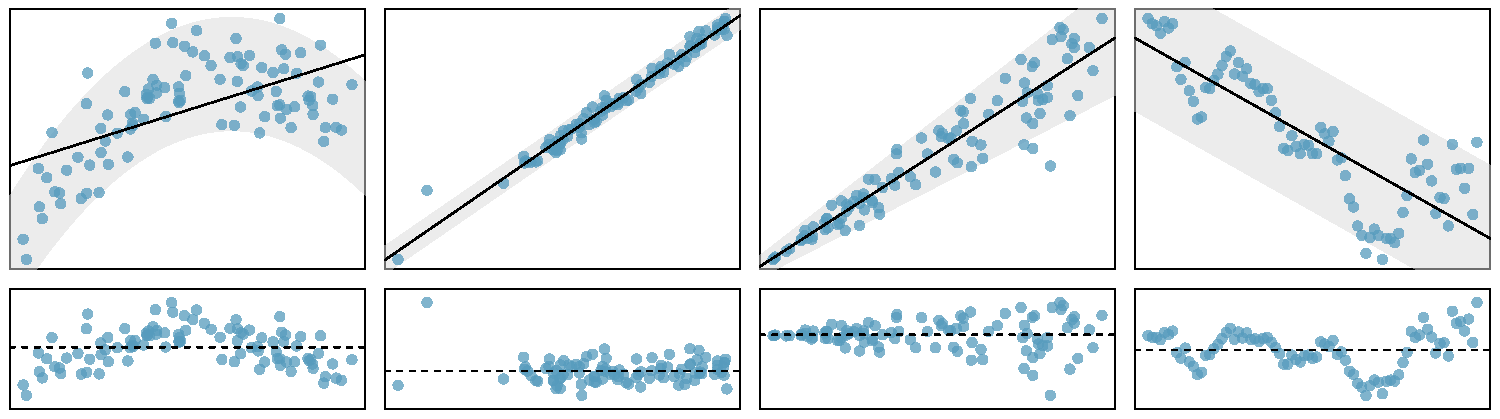
\includegraphics[width=\textwidth]{figures/whatCanGoWrongWithLinearModel/whatCanGoWrongWithLinearModel}
\end{figure}
\end{frame}

\begin{frame}{Least squares}
	\textbf{Least Squares regression}\\
	Choose the line that \textbf{minimises} the sum of the square residuals:
	\[e^1_1+e^2_2+\dots+e_n^2\]
	This is the \textbf{least square line}, with parameters
	\[b_0=\bar{y}-b_1\bar{x} \text{ and }b_1 = \frac{s_y}{s_x} R,\]
	where $\bar{x}$, $\bar{y}$, $s_x$, and $s_y$ are the sample means and standard deviations for each variable, and $b_0,b_1$ are the point estimates of $\beta_0$ and $\beta_1$ respectively.
\end{frame}
\begin{frame}{How to read the tables}
	\begin{figure}
	\centering
	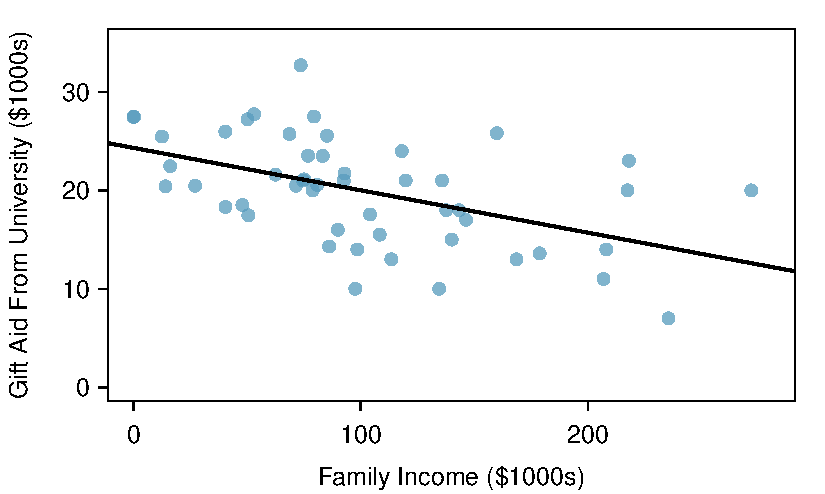
\includegraphics[width=0.7\textwidth]{figures/elmhurstPlots/elmhurstScatterWLSROnly}
	\end{figure}
	\resizebox{0.7\textwidth}{!}{
	\centering
	\begin{tabular}{l rrrr}
	  \hline
	  \vspace{-3.7mm} & & & & \\
	 & Estimate & Std. Error & t value & Pr($>$$|$t$|$) \\ 
	  \hline
	  \vspace{-3.6mm} & & & & \\
	(Intercept) & 24.3193 & 1.2915 & 18.83 & 0.0000 \\ 
	family\_\hspace{0.3mm}income & -0.0431 & 0.0108 & -3.98 & 0.0002 \\ 
	  \hline
	\end{tabular}}
\end{frame}
\begin{frame}{Interpreting regression}
	From the table $b_0=24.32$ and $b_1=-0.0431$, hence the least square line is:
	\[\hat{y} = 24.32 - 0.0431 x\]
	Or
	\[\widehat{aid} = 24.3 - 0.0431 \times family\_\hspace{0.3mm}income\]
	
\small	\textbf{Interpretation of slope} For each additional \$1,000 of family income, we would expect a student to receive a net difference of $\$\text{1,000}\times (-0.0431) = -\$43.10$ in aid on average, i.e. \$43.10 \emph{less}.\vspace{0.3cm}
	\textbf{Interpretation of intercept} The estimated intercept $b_0=24.3$ (in \$1000s) describes the average aid if a student's family had no income. 
\end{frame}
\begin{frame}{Strength of fit}
	%The quantity $s_y^2=\sum_{i=1}^n(y_i-\hat{y})^2$, provides a measure of total variation among the $y-$values. \\
	Sum of square errors:
	\[SSE=\sum_{i=1}^{n}(y_i-\hat{y}_i)^2\]
	\textbf{SSE} provides a measure of variation in the $y$ values that remains unexplained after using the linear regression model.\\
	\textbf{R-squared}
     \[R^2=1-\frac{SSE}{s_y^2}\]
\textbf{R-squared} can be interpreted as the proportion of the total variation in the $y$ values that is explained by the variable $x$ in least square line.

\textbf{Example:} For the Gift aid and family income data the correlation is $R=-0.499$ and the strength of fit is $R^2=0.25$.
\end{frame}
\begin{frame}{Extrapolation}
\small	\textbf{Extrapolation} is applying a model estimate to values outside the realm of the original data.\\
	
\textbf{Beware!!!}

\textbf{Example}\\
\small The fitted line for the gift aid at Elmhurst college, with respect to family income, is 

	\[\hat{y} = 24.32 - 0.0431 x\]

Can we predict the gift aid of a student with family income of \$ 1million?
\begin{itemize}
	\item Apply the model, the financial aid for the student is 
	\[\hat{y}=-18.8\]
	\item The student must pay extra -\$ 18.800
	\item This is unrealistic, since Elmhurst college only charges a tuition fee.
\end{itemize}
\end{frame}
\begin{frame}{Categorical predictors}
\small	Categorical variables can be incorporated in linear models.\\
	
\textbf{Data} Ebay auctions for a video game, \emph{Mario Kart} for the Nintendo Wii, where both the total price of the auction and the condition of the game were recorded.\\
\textbf{Goal} Fit a linear model of the form:\\
\[\widehat{price} = \beta_0 + \beta_1 \times \text{cond\_\hspace{0.3mm}new},\]
Formally, 
\[\hat{y}=\beta_0+\beta_1 x,\]
where $y$ is the price of the game in dollars and $x$ is a categorical variable, with $x=0$ if the game is used and $x=1$ if the game is new. 
\end{frame}
\begin{frame}{Categorical predictors}
	\begin{figure}
	\centering
	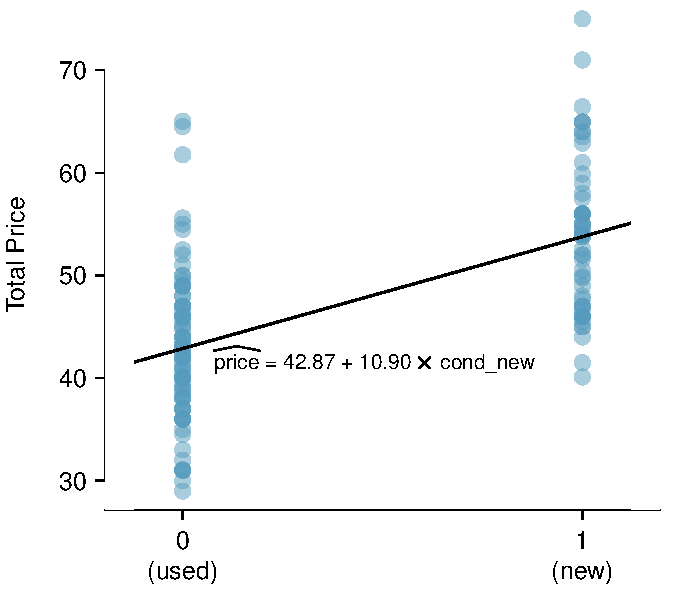
\includegraphics[width=0.65\textwidth]{figures/marioKartNewUsed/marioKartNewUsed}		  \end{figure}
	\end{frame}	
	\begin{frame}{Least square regression}
		\resizebox{0.7\textwidth}{!}{
		\begin{tabular}{rrrrr}
		  \hline
		  \vspace{-3.7mm} & & & & \\
		 & Estimate & Std. Error & t value & Pr($>$$|$t$|$) \\ 
		  \hline
		  \vspace{-3.6mm} & & & & \\
		(Intercept) & 42.87 & 0.81 & 52.67 & 0.0000 \\ 
		  cond\_\hspace{0.3mm}new & 10.90 & 1.26 & 8.66 & 0.0000 \\ 
		   \hline
		\end{tabular}}\\
		\textbf{Least square line}
		\[\hat{y}=42.87+10.9 x\]
		\textbf{Interpretation}
		\begin{itemize}
		 \item The intercept indicates that, the average selling price of a used version of the game is \$42.87.
		\item The slope indicates that, on average, new games sell for about \$10.90 more than used games.
	\end{itemize}
		\end{frame}
		\begin{frame}{Residuals}
			\begin{figure}
			\centering
			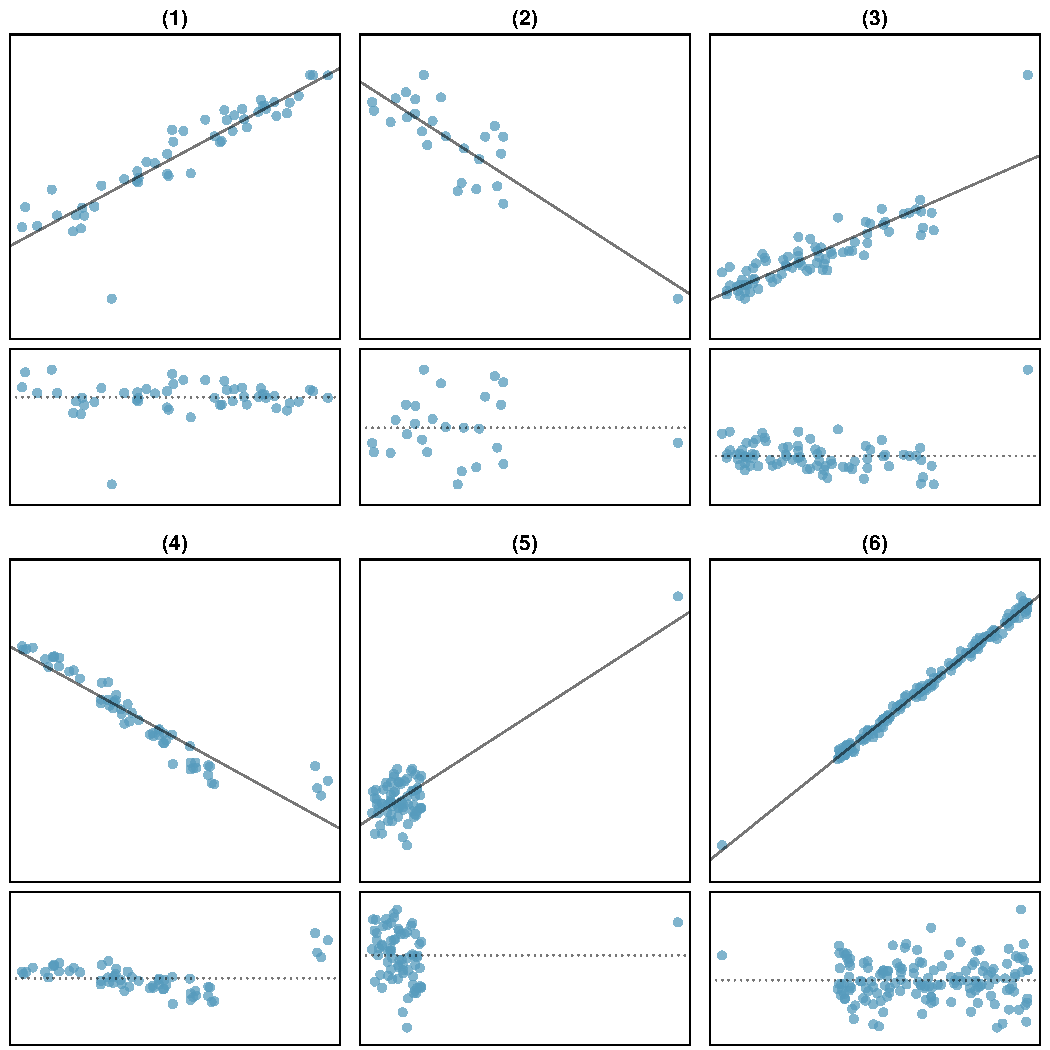
\includegraphics[width=0.7\textwidth]{figures/outlierPlots/outlierPlots}
	\end{figure}
			\end{frame}	
			\begin{frame}{Residuals}
			\small	\begin{itemize}
					\item Points that fall horizontally away from the centre of the cloud tend to pull harder on the line, so we call them points with \textbf{high leverage}.
\item If one of these high leverage points does appear to actually invoke its influence on the slope of the line  then we call it an \textbf{influential point}\footnote{ cases (3), (4), and (5)}.
\item If there are outliers in the data, they should not be removed or ignored without a~good reason. Whatever final model is fit to the data would not be very helpful if it ignores the most exceptional cases.
\item Be cautious about using a categorical predictor when one of the levels has very few observations. When this happens, those few observations become influential points.
				\end{itemize}
			\end{frame}
			\begin{frame}{Inference for linear regression}
				\textbf{Hypothesis:}  In America's two-party system, one political theory suggests the higher the unemployment rate, the worse the President's party will do in the midterm elections.
				\begin{figure}
				\centering
				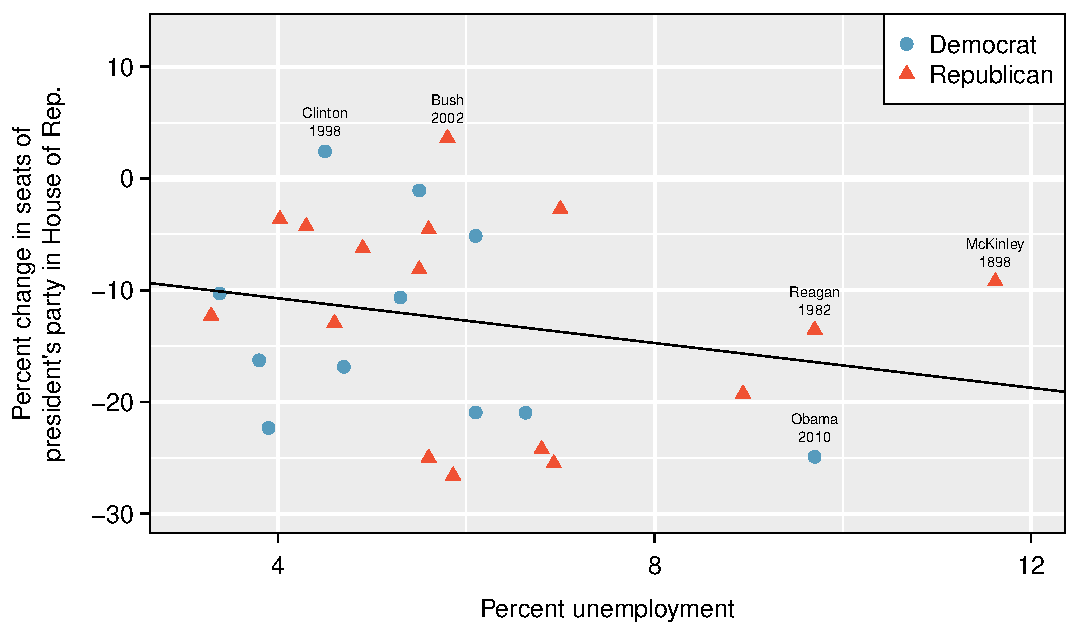
\includegraphics[width=0.95\textwidth]{figures/unemploymentAndChangeInHouse/unemploymentAndChangeInHouse}
			\end{figure}
			\end{frame}
			\begin{frame}{Read the tables}
					\resizebox{0.7\textwidth}{!}{
				\begin{tabular}{rrrrr}
				  \hline
				  \vspace{-3.7mm} & & & & \\
				 & Estimate & Std. Error & t value & Pr($>$$|$t$|$) \\ 
				  \hline
				  \vspace{-3.6mm} & & & & \\
				(Intercept) & -6.7142 & 5.4567 & -1.23 & 0.2300 \\ 
				  unemp & -1.0010 & 0.8717 & -1.15 & 0.2617 \\ 
				   \hline
				   \multicolumn{5}{r}{$df=25$} \\
				\end{tabular}}
				
			\textbf{Least square line}
				\[\hat{y} =-6.71 - 1.00 \times x,\]
			\small	where $y$ denotes the \% change in House seats for President's party and $x$ the unemployment rate.
			\end{frame}
			\begin{frame}{Hypothesis testing}
				\begin{itemize}
				\item[$H_0$:] $\beta_1 = 0$. 
				\item[$H_A$:] $\beta_1 < 0$. 
				\end{itemize}
				\textbf{Or}
				\begin{itemize}
				\item[$H_0$:] The true linear model has slope zero.
				\item[$H_A$:]The true linear model has a slope less than zero. The higher the unemployment, the greater the loss for the President's party in the House of Representatives.
				\end{itemize}
				\end{frame}
				\begin{frame}{Hypothesis Testing}
				\begin{itemize}
				\item From the table $P(>|t|)=0.2617$.\\
				\item For a one-sided test $p-value=P(>|t|)/2=0.13>0.05$
				\item There is no strong evidence to suggests that the higher the unemployment rate, the worse the President's party will do in the midterm elections.
				\end{itemize}
			\end{frame}
\end{document} 